%TC:group tabular 1 1
%TC:group table 1 1

\definecolor{bblue}{HTML}{4F81BD}
\definecolor{rred}{HTML}{C0504D}
\definecolor{ggreen}{HTML}{9BBB59}
\definecolor{ppurple}{HTML}{9F4C7C}
\definecolor{yyellow}{HTML}{CCAA40}
\definecolor{bbrown}{HTML}{662233}
\definecolor{excelGreen}{HTML}{50AA45}
\definecolor{sibPurple}{HTML}{822689}

\newcommand{\mycbox}[1]{\tikz{\path[draw=#1,fill=#1] (0,0) rectangle (0.3cm,0.3cm);}}

\chapter{Evaluation}

\paragraph{} This chapter Evaluates Excello against the success criteria and by showcasing examples. Converting of MIDI corpora to Excello using the converter demonstrates the notation's expressivity. Next, the summative evaluation is explained and its data used to assess the features implemented in the participatory design process and to reason about Excello using the CDN framework~\cite{blackwell:tutorial}. Finally, ethics and data handling procedures are covered.

\section{Excello Success}

\paragraph{} A musical notation and program integrated into Excel for playback have been implemented. As in the success criteria, users can play multiple notes and chords of different durations. These can be combined into looped sequences and have defined tempo. Additional features were added as extensions; multiple successive notes in a cell, turtles automatically moving forward and nested instructions with repeats all facilitate more efficient notation. Custom Excel functions, a chord adding tool and faster turtle toggling allows users to work more efficiently. Figure \ref{evaluation:excelloFranzRedacted} shows Excello in use with a participant's arrangement.

\begin{figure}[tbh]
\centerline{\includegraphics[width=150mm]{figs/excelloFranzRedacted.png}}
\caption{An arrangement with separated and labelled parts per instrument. Turtles refer to a global tempo at the top of the spreadsheet.}
\label{evaluation:excelloFranzRedacted}
\end{figure}

\paragraph{} The first section of Reich's Piano Phase is two identical piano melodies, one played slightly faster than the other. The parts move out of phas, periodically aligning at different offsets. This is included as an example for many end-user programming tools, perhaps as it cannot be concisely notated by western staff notation. Manhattan implements it using three rows of 24 columns~\cite{nash:manhattan}. Sonic Pi requires one line for the notes and eight for playback. Excello only requires two cells to define two turtles with different speeds in addition to the notes. All three implementations are shown in Figure \ref{evaluation:phase}.

\begin{figure}[!ht]
\begin{tabular}{cc}
  \multirow{3}{*}[2.72cm]{\includegraphics[width=65mm]{figs/manhattanPhase.png}} & \includegraphics[width=65mm]{figs/sonicPiPhase.png} \\
  & (b) The defined notes are played\\
  & by two concurrent loops with\\
  & different gaps between each note.\\[6pt]
  & \multirow{2}{*}{\includegraphics[width=65mm]{figs/excelloPhase.png}} \\
  (a) Column 01 keeps track of the phase,&\\
  02 defines the notes and 03 is the &\\
  phased notes - defined with formulae & (c) Two turtles play the same\\
  taking the phase and defined notes& notes at different speeds.\\
\end{tabular}
\caption{Implementations of Steve Reich's Piano Phase in (a) Manhattan, (b) Sonic Pi, (c) Excello}
\label{evaluation:phase}
\end{figure}

\section{MIDI Corpus Conversion}

\paragraph{} Whilst concisely notating some music western notation cannot, Excello can exactly express pieces defined in MIDI. Tempo being redefined within a track is not be accounted for. If instead the time between messages is adjusted, the uncompressed conversion accounts for this but the compressing algorithms will produce erroneous results as the difference between notes deviates too far from non-integer multiples of the minimum. Control messages like piano pedalling are not supported. Provided the difference between any two notes is a multiple of the minimum difference, the compression method that divides times by this accurately reproduces the MIDI, resulting in spreadsheets orders of magnitude smaller. This method would not accurately convert quavers against triplets (three notes played in the same time as two) provided these notes were not integer multiples of a smaller note. Given the lengths of MIDI notes can differ from the note's time in standard notation, an assumption on the ratio of note lengths was required for compression. The modal compressive conversion is lossy if the minimum note distance is not the modal distance. This is useful pieces with infrequently occuring ornaments or notes that dramatically decrease the minimum distance. Therefore this loss may be useful for more efficient representations.

\paragraph{} I have converted three MIDI corpora. A collection of 497 Bach chorales\footnote{Accessed from https://github.com/jamesrobertlloyd/infinite-bach/tree/master/data/chorales/midi.} made by Margaret Greentree, 280 piano pieces\footnote{http://piano-midi.de/midis.htm.} held by Bernd Krueger under a creative commons license,\footnote{https://creativecommons.org/licenses/by-sa/3.0/de/deed.en.} and 194 Bach pieces from ``A Johann Sebastian Bach Midi Page".\footnote{http://www.bachcentral.com/midiindex.html.} This is not all the files from this site as some were not readable using Mido. All 971 MIDI files were converted using all three methods.

\paragraph{} The Excello language is sufficiently expressive to represent MIDI files and can do so concisely provided the condition of minimum note onset differences is maintained.

\section{Summative Evaluation Sessions}

\paragraph{} 19 of the 21 participants continued using Excello after formative evaluation session and answered a summative evaluation questionnaire. First, the features added after the initial sessions were recapped. To ensure users sufficiently understood the interface before giving feedback, a short transcription task also requiring some authoring was given.

\paragraph{} The questionnaire first evaluated the participatory design process by comparing the interface before and after each feature. Seven-point Likert scale questions assessed if the issues had been solved and if overall the system was more preferable. The remaining questions were based on Blackwell and Greens' CDN questionnaire~\cite{blackwell:questionnaire}. CDN can be used to analyse musical notation~\cite{blackwell:notation} and software systems~\cite{green:cdn}, therefore it is suitable to discuss Excello's notation and interface. Dimensions significance for different activities varies~\cite{blackwell:tutorial}, so users identified the percentage of time they spent carrying out these activities (searching for information, translating, incrementation, modification and exploratory design). Likert scale questions focusing on closeness of mapping, consistency, secondary notation, viscosity and visibility were used as planned in the proposal. It was suspected that reasoning about cognitive dimensions would be more challenging for participants, so to reduce the expected variance, only a five-point Likert scale was used. The two have been shown to produce similar results~\cite{dawes:points}. CDN results were also collected for the user's preferred music composition interface. 12 users chose Sibelius, which shall be used for comparison.

\section{Success of Participatory Design}

\paragraph{} For each feature added, Excello with (system 2) and without this feature were compared. The following charts show the Likert scale responses for each question. I considered the mode of the Likert scale~\cite{barry:likert}. Chi-squared goodness-of-fit tests confirm the distributions are significantly different to uniform. All expected values must be greater than 1 and 80\% greater than or equal to five~\cite{ross:introductory}. As the expected frequency for one result is $19/7 \approx 2.7$, I combine Strongly Disagree with Disagree, Strongly Agree with Agree and the remaining three options into a third group. The p-value from a chi-squared test with these categories is given.

\subsection{Dynamics in the Cell}

\begin{table}[!htbp]
\centering
% \caption{Grammar rules for turtle movement instructions. $z \in \mathbb{Z}, n \in \mathbb{N}, c \in \texttt{[A-Za-z]}^{+}$.}
\vspace{1pt}
\begin{tabular}{|l|l|l|} \hline
\textbf{Statement}&\textbf{Mode}&\textbf{p-value}\\ \hline
\mycbox{bblue} It is easier to figure out the turtle's path.&Strongly Agree&0.0000\\ \hline
\mycbox{rred} It is easier to figure out what dynamics different&Strongly Agree&0.0146\\
notes are played at.&&\\ \hline
\mycbox{ggreen} It is easier to tell the order in which dynamics are applied.&Strongly Agree&0.0000\\ \hline
\mycbox{ppurple} It is easier to write dynamics in the correct place.&Strongly Agree&0.0000\\ \hline
\mycbox{yyellow} Overall system 2 is preferable.&Strongly Agree&0.0000 \\ \hline
\end{tabular}
\label{evaluation:cellDynamics}
\end{table}

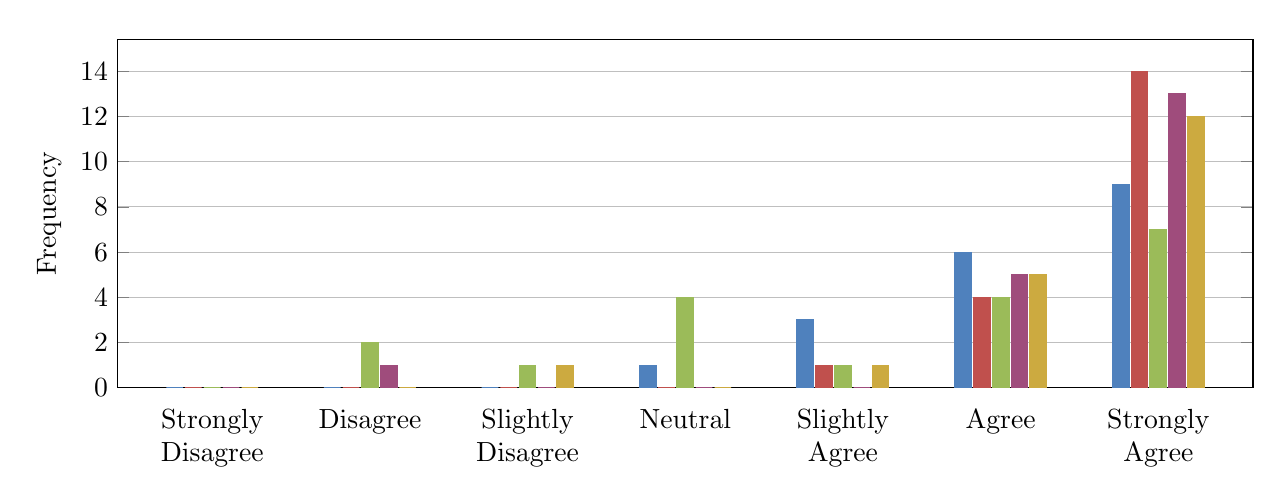
\begin{tikzpicture}
    \begin{axis}[
      % width  = \textwidth,
      width = 16cm,
      height = 6cm,
      major x tick style = transparent,
      ybar=2*\pgflinewidth,
      bar width=6pt,
      ymajorgrids = true,
      ylabel = {Frequency},
      %xlabel = {Likert Scale Result},
      symbolic x coords= {-3,-2,-1,0,1,2,3},
      xticklabels = {Strongly Disagree,Disagree,Slightly Disagree,Neutral,Slightly Agree,Agree,Strongly Agree},
      xtick = data,
      ytick = {0,2,4,6,8,10,12,14},
      x tick label style  = {text width=2cm,align=center},
      scaled y ticks = false,
      % enlarge x limits=0.25,
      ymin=0,
      legend cell align=left,
      legend style={
              at={(1,1.05)},
              anchor=south east,
              column sep=1ex
      }
    ]
        \addplot[style={bblue,fill=bblue,mark=none}]
            coordinates {(-3,0) (-2,0) (-1,0) (0,1) (1,3) (2,6) (3,9) };

        \addplot[style={rred,fill=rred,mark=none}]
             coordinates {(-3,0) (-2,0) (-1,0) (0,0) (1,1) (2,4) (3,14) };

        \addplot[style={ggreen,fill=ggreen,mark=none}]
             coordinates {(-3,0) (-2,2) (-1,1) (0,4) (1,1) (2,4) (3,7) };

        \addplot[style={ppurple,fill=ppurple,mark=none}]
             coordinates {(-3,0) (-2,1) (-1,0) (0,0) (1,0) (2,5) (3,13) };

       \addplot[style={yyellow,fill=yyellow,mark=none}]
           coordinates {(-3,0) (-2,0) (-1,1) (0,0) (1,1) (2,5) (3,12) };

        % \legend{It is easier to figure out the turtles path,It is easier to figure out what dynamics different notes are played at,It is easier to tell the order in which dynamics are applied,It is easier to write dynamics in the correct place,Overall system 2 is preferable}
    \end{axis}
\end{tikzpicture}

\paragraph{} There is strong evidence suggesting this change improved some of the issues identified during participatory design, resulting in an improved system.

\subsection{Inferred Octave}
\ %This is here to put the section heading and table in the right order

\begin{table}[!ht]
\centering
% \caption{Grammar rules for turtle movement instructions. $z \in \mathbb{Z}, n \in \mathbb{N}, c \in \texttt{[A-Za-z]}^{+}$.}
\vspace{1pt}
\begin{tabular}{|l|l|l|} \hline
\textbf{Statement}&\textbf{Mode}&\textbf{p-value}\\ \hline
\mycbox{bblue} Less effort is required to write a part.&Strongly Agree&0.0000 \\ \hline
\mycbox{rred} It is harder to figure out what octave a note will be&Slightly Agree&0.0639 \\
played in.&& \\ \hline
\mycbox{ggreen} Overall, system 2 is preferable.&Strongly Agree&0.0000 \\ \hline
\end{tabular}
\label{evaluation:inferredOctave}
\end{table}

\vspace{10pt}
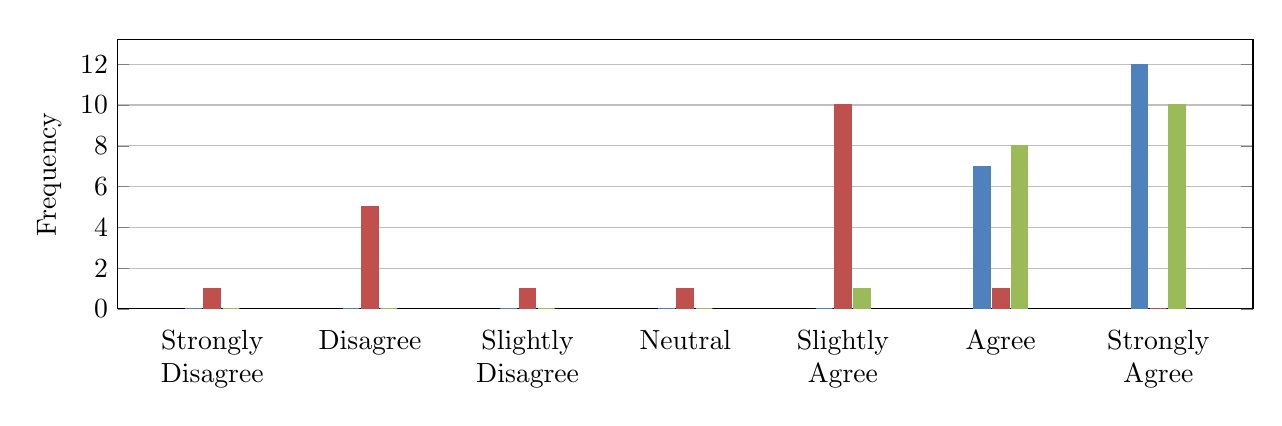
\begin{tikzpicture}
    \begin{axis}[
      width  = 16cm,
      height = 5cm,
      major x tick style = transparent,
      ybar=2*\pgflinewidth,
      bar width=6pt,
      ymajorgrids = true,
      ylabel = {Frequency},
      %xlabel = {Likert Scale Result},
      symbolic x coords= {-3,-2,-1,0,1,2,3},
      xticklabels = {Strongly Disagree,Disagree,Slightly Disagree,Neutral,Slightly Agree,Agree,Strongly Agree},
      xtick = data,
      ytick = {0,2,4,6,8,10,12,14},
      x tick label style  = {text width=2cm,align=center},
      scaled y ticks = false,
      % enlarge x limits=0.25,
      ymin=0,
      legend cell align=left,
      legend style={
              at={(1,1.05)},
              anchor=south east,
              column sep=1ex
      }
    ]
    \addplot[style={bblue,fill=bblue,mark=none}]
    	coordinates {(-3,0) (-2,0) (-1,0) (0,0) (1,0) (2,7) (3,12) };
    \addplot[style={rred,fill=rred,mark=none}]
    	coordinates {(-3,1) (-2,5) (-1,1) (0,1) (1,10) (2,1) (3,0) };
    \addplot[style={ggreen,fill=ggreen,mark=none}]
    	coordinates {(-3,0) (-2,0) (-1,0) (0,0) (1,1) (2,8) (3,10) };

    \end{axis}
\end{tikzpicture}

% \vspace{-20pt}
\paragraph{} The inferred octave notation makes octaves harder to infer. However, the response distribution is not significantly different to uniform at the 5\% level. Overall this addition was significantly preferable.

\subsection{Nested Instructions}

\begin{table}[!htbp]
\centering
% \caption{Grammar rules for turtle movement instructions. $z \in \mathbb{Z}, n \in \mathbb{N}, c \in \texttt{[A-Za-z]}^{+}$.}
\vspace{1pt}
\begin{tabular}{|l|l|l|} \hline
\textbf{Statement}&\textbf{Mode}&\textbf{p-value}\\ \hline
\mycbox{bblue} It is easier to parse the turtle instruction and tell &Agree&0.0003\\
what it will do.&& \\ \hline
\mycbox{rred} It is easier to repeat sections of notes.&Strongly Agree&0.0000\\ \hline
\mycbox{ggreen} Overall, system 2 is preferable.&Strongly Agree&0.0000\\ \hline
\end{tabular}
\label{evaluation:nestedInstructions}
\end{table}

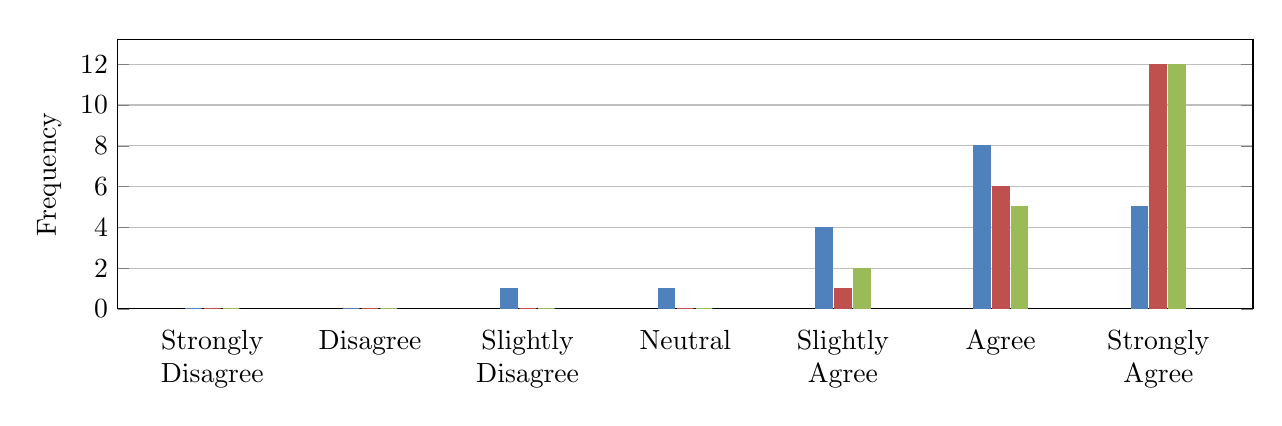
\begin{tikzpicture}
    \begin{axis}[
      % width  = \textwidth,
      width = 16cm,
      height = 5cm,
      major x tick style = transparent,
      ybar=2*\pgflinewidth,
      bar width=6pt,
      ymajorgrids = true,
      ylabel = {Frequency},
      %xlabel = {Likert Scale Result},
      symbolic x coords= {-3,-2,-1,0,1,2,3},
      xticklabels = {Strongly Disagree,Disagree,Slightly Disagree,Neutral,Slightly Agree,Agree,Strongly Agree},
      xtick = data,
      ytick = {0,2,4,6,8,10,12,14},
      x tick label style  = {text width=2cm,align=center},
      scaled y ticks = false,
      % enlarge x limits=0.25,
      ymin=0,
      legend cell align=left,
      legend style={
              at={(1,1.05)},
              anchor=south east,
              column sep=1ex
      }
    ]
    \addplot[style={bblue,fill=bblue,mark=none}]
    coordinates {(-3,0) (-2,0) (-1,1) (0,1) (1,4) (2,8) (3,5) };
    \addplot[style={rred,fill=rred,mark=none}]
    coordinates {(-3,0) (-2,0) (-1,0) (0,0) (1,1) (2,6) (3,12) };
    \addplot[style={ggreen,fill=ggreen,mark=none}]
    coordinates {(-3,0) (-2,0) (-1,0) (0,0) (1,2) (2,5) (3,12) };

        % \legend{It is easier to figure out the turtles path,It is easier to figure out what dynamics different notes are played at,It is easier to tell the order in which dynamics are applied,It is easier to write dynamics in the correct place,Overall system 2 is preferable}
    \end{axis}
\end{tikzpicture}

\paragraph{} All participants found the addition of nested instructions with repeats preferable, with the majority strongly agreeing.

\subsection{Active Turtles List}

\begin{table}[!htbp]
\centering
% \caption{Grammar rules for turtle movement instructions. $z \in \mathbb{Z}, n \in \mathbb{N}, c \in \texttt{[A-Za-z]}^{+}$.}
\vspace{1pt}
\begin{tabular}{|l|l|l|} \hline
\textbf{Statement}&\textbf{Mode}&\textbf{p-value}\\ \hline
\mycbox{bblue} It is easier to tell if a certain turtle has been registered.&Strongly Agree&0.0000\\ \hline
\mycbox{rred} It is easier to see where the active turtles are.&(Strongly) Agree&0.0011\\\hline
\mycbox{ggreen} It is easier to toggle the activation of turtles.&Agree&0.0038 \\ \hline
\mycbox{ppurple} Overall, system 2 is preferable.&Strongly Agree&0.0000 \\ \hline
\end{tabular}
\label{evaluation:activeTurtles}
\end{table}

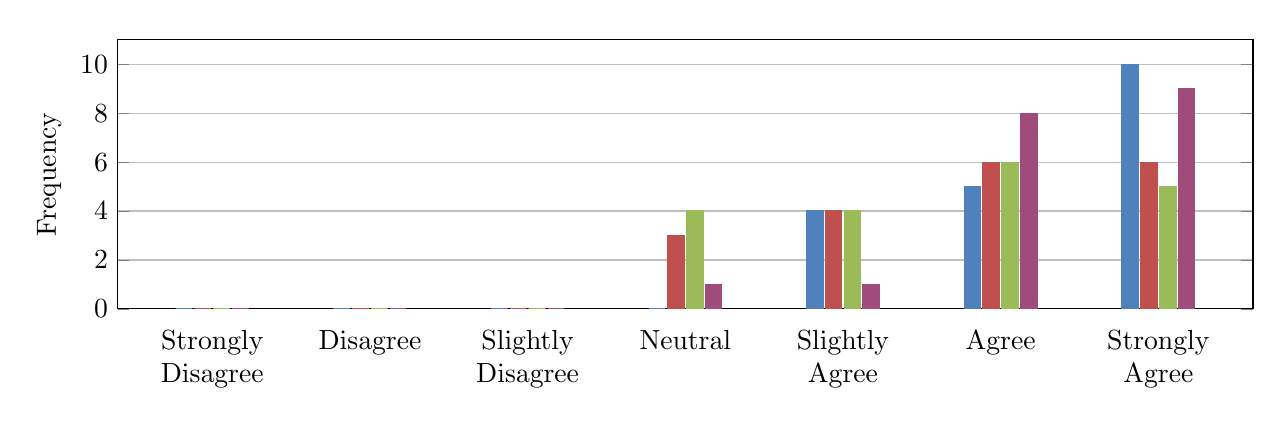
\begin{tikzpicture}
    \begin{axis}[
      % width  = \textwidth,
      width = 16cm,
      height = 5cm,
      major x tick style = transparent,
      ybar=2*\pgflinewidth,
      bar width=6pt,
      ymajorgrids = true,
      ylabel = {Frequency},
      %xlabel = {Likert Scale Result},
      symbolic x coords= {-3,-2,-1,0,1,2,3},
      xticklabels = {Strongly Disagree,Disagree,Slightly Disagree,Neutral,Slightly Agree,Agree,Strongly Agree},
      xtick = data,
      ytick = {0,2,4,6,8,10,12,14},
      x tick label style  = {text width=2cm,align=center},
      scaled y ticks = false,
      % enlarge x limits=0.25,
      ymin=0,
      legend cell align=left,
      legend style={
              at={(1,1.05)},
              anchor=south east,
              column sep=1ex
      }
    ]
    \addplot[style={bblue,fill=bblue,mark=none}]
    coordinates {(-3,0) (-2,0) (-1,0) (0,0) (1,4) (2,5) (3,10) };
    \addplot[style={rred,fill=rred,mark=none}]
    coordinates {(-3,0) (-2,0) (-1,0) (0,3) (1,4) (2,6) (3,6) };
    \addplot[style={ggreen,fill=ggreen,mark=none}]
    coordinates {(-3,0) (-2,0) (-1,0) (0,4) (1,4) (2,6) (3,5) };
    \addplot[style={ppurple,fill=ppurple,mark=none}]
    coordinates {(-3,0) (-2,0) (-1,0) (0,1) (1,1) (2,8) (3,9) };

        % \legend{It is easier to figure out the turtles path,It is easier to figure out what dynamics different notes are played at,It is easier to tell the order in which dynamics are applied,It is easier to write dynamics in the correct place,Overall system 2 is preferable}
    \end{axis}
\end{tikzpicture}

\paragraph{} A list of active turtles had a neutral or positive effect for all users.

\subsection{Continuous Volume}

\begin{table}[!htbp]
\centering
% \caption{Grammar rules for turtle movement instructions. $z \in \mathbb{Z}, n \in \mathbb{N}, c \in \texttt{[A-Za-z]}^{+}$.}
\vspace{1pt}
\begin{tabular}{|l|l|l|} \hline
\textbf{Statement}&\textbf{Mode}&\textbf{p-value}\\ \hline
\mycbox{bblue} It is more intuitive how loud a note will be played.&Disagree&0.6592\\
&Strongly Agree& \\ \hline
\mycbox{rred} The volumes available are less limited.&Strongly Agree&0.0000\\ \hline
\mycbox{ggreen} Overall, system 2 is preferable.&Agree&0.0003\\ \hline
\end{tabular}
\label{evaluation:continuousVolume}
\end{table}

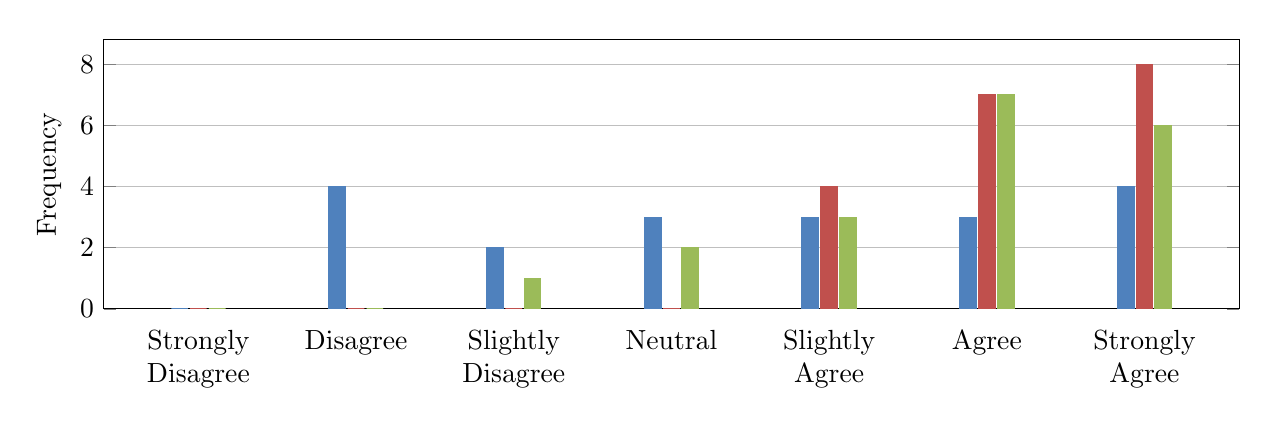
\begin{tikzpicture}
    \begin{axis}[
      % width  = \textwidth,
      width = 16cm,
      height = 5cm,
      major x tick style = transparent,
      ybar=2*\pgflinewidth,
      bar width=6pt,
      ymajorgrids = true,
      ylabel = {Frequency},
      %xlabel = {Likert Scale Result},
      symbolic x coords= {-3,-2,-1,0,1,2,3},
      xticklabels = {Strongly Disagree,Disagree,Slightly Disagree,Neutral,Slightly Agree,Agree,Strongly Agree},
      xtick = data,
      ytick = {0,2,4,6,8,10,12,14},
      x tick label style  = {text width=2cm,align=center},
      scaled y ticks = false,
      % enlarge x limits=0.25,
      ymin=0,
      legend cell align=left,
      legend style={
              at={(1,1.05)},
              anchor=south east,
              column sep=1ex
      }
    ]
    \addplot[style={bblue,fill=bblue,mark=none}]
    coordinates {(-3,0) (-2,4) (-1,2) (0,3) (1,3) (2,3) (3,4) };
    \addplot[style={rred,fill=rred,mark=none}]
    coordinates {(-3,0) (-2,0) (-1,0) (0,0) (1,4) (2,7) (3,8) };
    \addplot[style={ggreen,fill=ggreen,mark=none}]
    coordinates {(-3,0) (-2,0) (-1,1) (0,2) (1,3) (2,7) (3,6) };

        % \legend{It is easier to figure out the turtles path,It is easier to figure out what dynamics different notes are played at,It is easier to tell the order in which dynamics are applied,It is easier to write dynamics in the correct place,Overall system 2 is preferable}
    \end{axis}
\end{tikzpicture}

\paragraph{} There is no significant result for whether the ability to define volume in the range [0,1] is more intuitive. All users agreed that the volumes were less confined. However, only one user did not find this change preferable. Given the previous conventional dynamic markings can still be used, this supports the addition being successful.

\subsection{Automatic Stepping}

\begin{table}[!htbp]
\centering
% \caption{Grammar rules for turtle movement instructions. $z \in \mathbb{Z}, n \in \mathbb{N}, c \in \texttt{[A-Za-z]}^{+}$.}
\vspace{1pt}
\begin{tabular}{|l|l|l|} \hline
\textbf{Statement}&\textbf{Mode}&\textbf{p-value}\\ \hline
\mycbox{bblue} Less mental work is required to write the turtle. &Strongly Agree&0.0000\\
instructions.&& \\ \hline
\mycbox{rred} Less work is required when more notes wish to be added.&Strongly Agree&0.0000\\ \hline
\mycbox{ggreen} Overall, system 2 is preferable.&Strongly Agree&0.0000\\ \hline
\end{tabular}
\label{evaluation:automaticStepping}
\end{table}

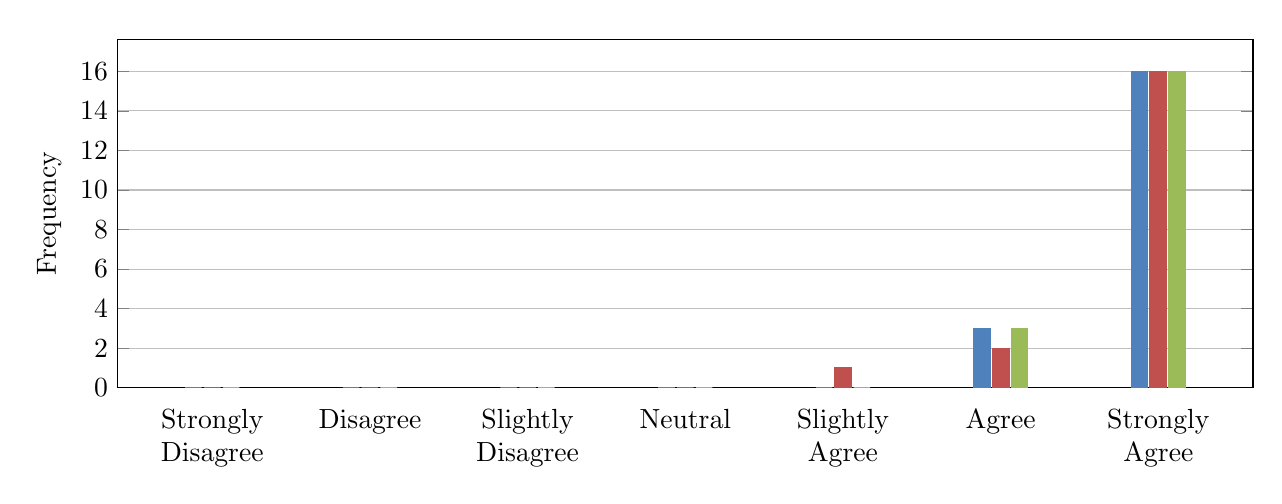
\begin{tikzpicture}
    \begin{axis}[
      % width  = \textwidth,
      width = 16cm,
      height = 6cm,
      major x tick style = transparent,
      ybar=2*\pgflinewidth,
      bar width=6pt,
      ymajorgrids = true,
      ylabel = {Frequency},
      %xlabel = {Likert Scale Result},
      symbolic x coords= {-3,-2,-1,0,1,2,3},
      xticklabels = {Strongly Disagree,Disagree,Slightly Disagree,Neutral,Slightly Agree,Agree,Strongly Agree},
      xtick = data,
      ytick = {0,2,4,6,8,10,12,14,16},
      x tick label style  = {text width=2cm,align=center},
      scaled y ticks = false,
      % enlarge x limits=0.25,
      ymin=0,
      legend cell align=left,
      legend style={
              at={(1,1.05)},
              anchor=south east,
              column sep=1ex
      }
    ]
    \addplot[style={bblue,fill=bblue,mark=none}]
    coordinates {(-3,0) (-2,0) (-1,0) (0,0) (1,0) (2,3) (3,16) };
    \addplot[style={rred,fill=rred,mark=none}]
    coordinates {(-3,0) (-2,0) (-1,0) (0,0) (1,1) (2,2) (3,16) };
    \addplot[style={ggreen,fill=ggreen,mark=none}]
    coordinates {(-3,0) (-2,0) (-1,0) (0,0) (1,0) (2,3) (3,16) };

        % \legend{It is easier to figure out the turtles path,It is easier to figure out what dynamics different notes are played at,It is easier to tell the order in which dynamics are applied,It is easier to write dynamics in the correct place,Overall system 2 is preferable}
    \end{axis}
\end{tikzpicture}

\paragraph{} This feature was particularly successful with 16 of the 19 users strongly agreeing the system was more preferable with automatic stepping available in the turtle instructions.

\subsection{Absolute Tempo}

\begin{table}[!htbp]
\centering
% \caption{Grammar rules for turtle movement instructions. $z \in \mathbb{Z}, n \in \mathbb{N}, c \in \texttt{[A-Za-z]}^{+}$.}
\vspace{1pt}
\begin{tabular}{|l|l|l|} \hline
\textbf{Statement}&\textbf{Mode}&\textbf{p-value}\\ \hline
\mycbox{bblue} It is easier to tell what the speed instruction&Strongly Agree&0.0000\\
 corresponds to.&& \\ \hline
\mycbox{rred} Giving an exact tempo (e.g.~when transcribing sheet&Strongly Agree&0.0000\\
music) is easier.&& \\ \hline
\mycbox{ggreen} Overall, system 2 is preferable.&Strongly Agree&0.0000\\ \hline
\end{tabular}
\label{evaluation:absoluteTempo}
\end{table}

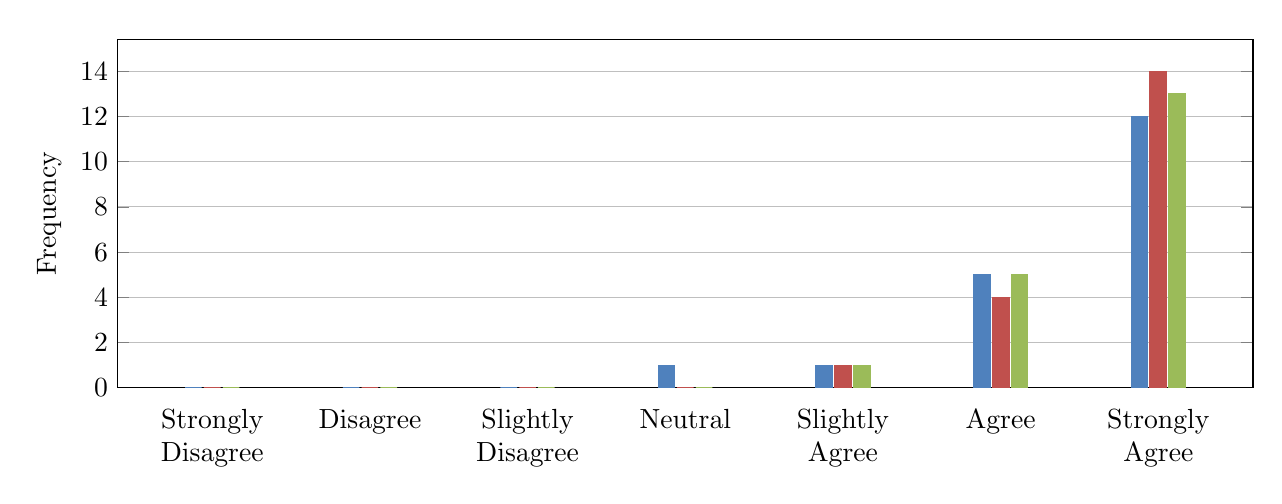
\begin{tikzpicture}
    \begin{axis}[
      % width  = \textwidth,
      width = 16cm,
      height = 6cm,
      major x tick style = transparent,
      ybar=2*\pgflinewidth,
      bar width=6pt,
      ymajorgrids = true,
      ylabel = {Frequency},
      %xlabel = {Likert Scale Result},
      symbolic x coords= {-3,-2,-1,0,1,2,3},
      xticklabels = {Strongly Disagree,Disagree,Slightly Disagree,Neutral,Slightly Agree,Agree,Strongly Agree},
      xtick = data,
      ytick = {0,2,4,6,8,10,12,14},
      x tick label style  = {text width=2cm,align=center},
      scaled y ticks = false,
      % enlarge x limits=0.25,
      ymin=0,
      legend cell align=left,
      legend style={
              at={(1,1.05)},
              anchor=south east,
              column sep=1ex
      }
    ]
    \addplot[style={bblue,fill=bblue,mark=none}]
    coordinates {(-3,0) (-2,0) (-1,0) (0,1) (1,1) (2,5) (3,12) };
    \addplot[style={rred,fill=rred,mark=none}]
    coordinates {(-3,0) (-2,0) (-1,0) (0,0) (1,1) (2,4) (3,14) };
    \addplot[style={ggreen,fill=ggreen,mark=none}]
    coordinates {(-3,0) (-2,0) (-1,0) (0,0) (1,1) (2,5) (3,13) };

        % \legend{It is easier to figure out the turtles path,It is easier to figure out what dynamics different notes are played at,It is easier to tell the order in which dynamics are applied,It is easier to write dynamics in the correct place,Overall system 2 is preferable}
    \end{axis}
\end{tikzpicture}

\paragraph{} The initial design was changed so that turtle speed was defined in absolute cells per minute. All users found this to be an improvement.

\paragraph{} Overall, the participatory design process was very successful. Multiple features were added to Excello to solve problems identified through formative evaluation sessions and longer-term user feedback. There is significant evidence that all added features improved Excello.

\section{Cognitive Dimensions of Notation}

\paragraph{} Figure \ref{fig:usage} shows the time users identified carrying out the different cognitive activities~\cite{blackwell:tutorial} in Excello and in Sibelius. There are 19 Excello users and 12 for Sibelius. This shows translation is very important for both interfaces. There is more exploratory design for Excello but as users become more familiar with the system and more Excello notation exists, modification and incrementation may become more important. Little time is spent searching for information in the notation in either.

\begin{figure}[ht]
\centering
\begin{subfigure}{.6\textwidth}
  \centering
    \begin{tikzpicture}
      \begin{axis}
        [
        height = 6cm,
        width = 7cm,
        ytick={1,2,3,4,5},
        yticklabels={Searching, Translation, Incrementation, Modification, Exploratory Design},
        xlabel = {Percentage of Time}
        ]
        \addplot+[
        	boxplot prepared={
        		median=10,
        		upper quartile=3.319672131,
        		lower quartile=10,
        		upper whisker=30,
        		lower whisker=0
        	},
        ] coordinates {};
        \addplot+[
        	boxplot prepared={
        		median=50,
        		upper quartile=45,
        		lower quartile=65,
        		upper whisker=100,
        		lower whisker=8
        	},
        ] coordinates {};
        \addplot+[
        	boxplot prepared={
        		median=10,
        		upper quartile=5,
        		lower quartile=15.69672131,
        		upper whisker=24,
        		lower whisker=0
        	},
        ] coordinates {};
        \addplot+[
        	boxplot prepared={
        		median=10,
        		upper quartile=5,
        		lower quartile=15.69672131,
        		upper whisker=30,
        		lower whisker=0
        	},
        ] coordinates {};
        \addplot+[
        	boxplot prepared={
        		median=10,
        		upper quartile=9,
        		lower quartile=27,
        		upper whisker=49,
        		lower whisker=0
        	},
        ] coordinates {};
      \end{axis}
    \end{tikzpicture}
  % \caption{A subfigure}
  \label{fig:sub1}
\end{subfigure}%
\begin{subfigure}{.4\textwidth}
  \centering
    \begin{tikzpicture}
      \begin{axis}
        [
        height = 6cm,
        width = 6.5cm,
        ytick={1,2,3,4,5},
        yticklabels={},
        xlabel = {Percentage of Time}
        ]
        \addplot+[
          boxplot prepared={
            median=10,
            upper quartile=5,
            lower quartile=11,
            upper whisker=27.27272727,
            lower whisker=0.460829493
          },
        ] coordinates {};
        \addplot+[
          boxplot prepared={
            median=40.22727273,
            upper quartile=30,
            lower quartile=50,
            upper whisker=60,
            lower whisker=13.82488479
          },
        ] coordinates {};
        \addplot+[
          boxplot prepared={
            median=20,
            upper quartile=15,
            lower quartile=29.25,
            upper whisker=41.47465438,
            lower whisker=4.545454545
          },
        ] coordinates {};
        \addplot+[
          boxplot prepared={
            median=16.09090909,
            upper quartile=10,
            lower quartile=30,
            upper whisker=41.47465438,
            lower whisker=5
          },
        ] coordinates {};
        \addplot+[
          boxplot prepared={
            median=9.166666667,
            upper quartile=4.886363636,
            lower quartile=15,
            upper whisker=20,
            lower whisker=0
          },
        ] coordinates {};
      \end{axis}
    \end{tikzpicture}
  % \caption{A subfigure}
  \label{fig:sub2}
\end{subfigure}
\caption{The percentage of time spent performing the different cognitive activities in Excello (left) and Sibelius (right).}
\label{fig:usage}
\end{figure}

\vspace{-20pt}
\paragraph{} A series of statements from~\cite{blackwell:questionnaire} were selected to assess the CDN of Excello. Users responded with a five-point (Strongly Disagree, Disagree, Neutral, Agree, Strongly Agree) Likert scale. The significance of the results was verified with a chi-squared test. First, the data was combined into negative and non-negative categories. For each statement, the chi-squared test p-value and modal response are shown in Table \ref{evaluation:cdnTable}. The distribution of responses is shown in Figure \ref{evaluation:cdnQuestions}.

\begin{table}[!htbp]
\centering
\vspace{1pt}
\begin{tabular}{|l|l|l|l|} \hline
\textbf{Statement}&\textbf{CDN}&\textbf{Mode}&\textbf{p-value}\\ \hline
\mycbox{bblue} (a) The notation used (In Excello: notes/ &Closeness&Agree&0.0004\\
dynamics in cells and the definition of turtles)&of&& \\
is related to the result you are describing (In &Mapping&& \\
Excello: Musical output)&&& \\ \hline
\mycbox{rred} (b) Where there are different parts of the&Consistency&Agree&0.0087\\
notation that mean similar things, the&&& \\
similarity is clear from the way they appear. &&& \\ \hline
\mycbox{ggreen} (c) You can add extra marks (or colours or &Secondary&Agree&0.0020\\
format choices) to clarify, emphasise or repeat&Notation&& \\
what is there already. &&& \\ \hline
\mycbox{ppurple} (d) When you need to make changes to&Viscosity&Agree&0.0004 \\
previous, work it is easy to make the change.&&& \\ \hline
\mycbox{yyellow} (e) It is easy to see or find the various parts of &Visibility/&Agree&0.0087 \\
the notation while it is being created or changed.&Juxtaposition&& \\ \hline
\mycbox{bbrown} (f) If you need to compare or combine different&Visibility/&Agree&0.0312 \\
parts, you can see them at the same time.&Juxtaposition&& \\ \hline
\end{tabular}
\caption{Questions and results for testing the CDN of Excello \label{evaluation:cdnTable}}
\end{table}

\begin{figure} [!htbp]
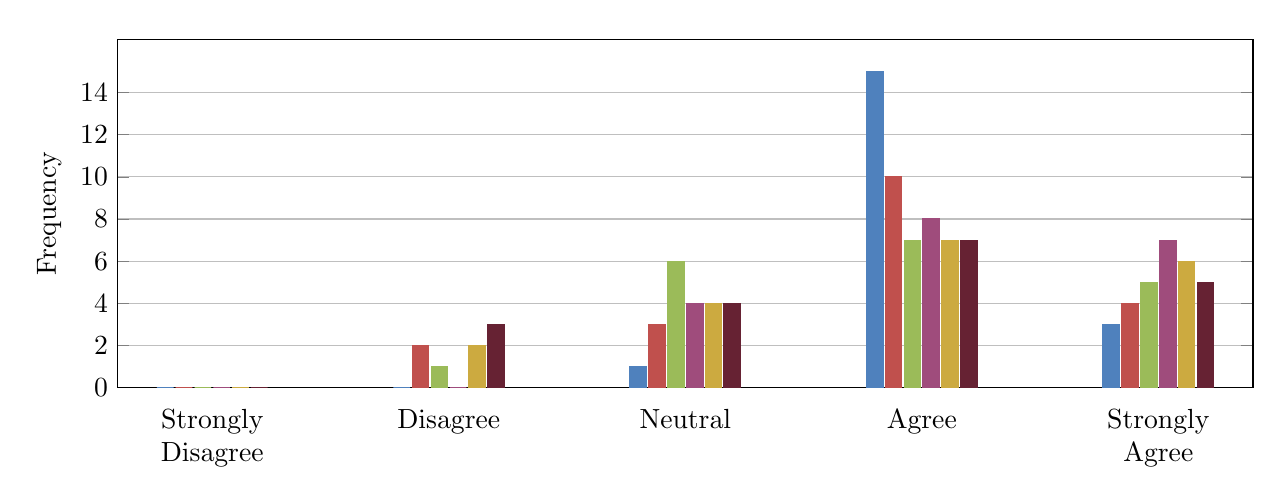
\begin{tikzpicture}
    \begin{axis}[
      % width  = \textwidth,
      width = 16cm,
      height = 6cm,
      major x tick style = transparent,
      ybar=2*\pgflinewidth,
      bar width=6pt,
      ymajorgrids = true,
      ylabel = {Frequency},
      %xlabel = {Likert Scale Result},
      symbolic x coords= {-3,-2,-1,0,1,2,3},
      xticklabels = {Strongly Disagree,Disagree,Neutral,Agree,Strongly Agree},
      xtick = data,
      ytick = {0,2,4,6,8,10,12,14},
      x tick label style  = {text width=2cm,align=center},
      scaled y ticks = false,
      % enlarge x limits=0.25,
      ymin=0,
      legend cell align=left,
      legend style={
              at={(1,1.05)},
              anchor=south east,
              column sep=1ex
      }
    ]
    \addplot[style={bblue,fill=bblue,mark=none}]
    	coordinates {(-3,0) (-2,0) (-1,1) (0,15) (1,3) };
    \addplot[style={rred,fill=rred,mark=none}]
    	coordinates {(-3,0) (-2,2) (-1,3) (0,10) (1,4) };
    \addplot[style={ggreen,fill=ggreen,mark=none}]
    	coordinates {(-3,0) (-2,1) (-1,6) (0,7) (1,5) };
    \addplot[style={ppurple,fill=ppurple,mark=none}]
    	coordinates {(-3,0) (-2,0) (-1,4) (0,8) (1,7) };
    \addplot[style={yyellow,fill=yyellow,mark=none}]
    	coordinates {(-3,0) (-2,2) (-1,4) (0,7) (1,6) };
    \addplot[style={bbrown,fill=bbrown,mark=none}]
    	coordinates {(-3,0) (-2,3) (-1,4) (0,7) (1,5) };

    \end{axis}
\end{tikzpicture}
\caption{The responses to the questions in Table \ref{evaluation:cdnTable}}
\label{evaluation:cdnQuestions}
\end{figure}

\paragraph{} As these questions were also answered for the user's preferred interface, a comparison to Sibelius is made. As the data does not meet the assumptions of the t-test~\cite{barry:likert}, I performed a Wilcoxon matched pairs signed-ranked test on the 12 pairs by encoding the five responses as -2,-1,0,1,2. For all six questions, there is no indication that the answers for the two interfaces come from populations with different means.

\subsection{Closeness of Mapping}

\paragraph{} A test value of 5 for 5 changed pairs provides no significant evidence that the population means for Excello and Sibelius were different, suggesting Excello's notation with spreadsheets has not compromised the closeness of mapping of traditional notation. This is helped by using existing SPN for defining notes, the turtle instructions mapping to movement through the grid, and by the speed argument being an absolute, not relative, parameter. Being less familiar with staff notation, user 4 had found Sibelius's notation unintuitive.

\begin{figure}[htb]
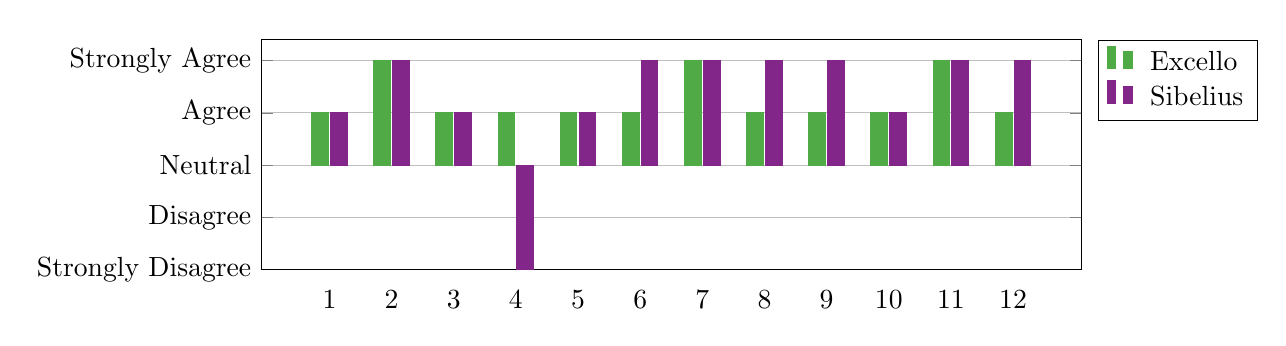
\begin{tikzpicture}
    \begin{axis}[
      % width  = \textwidth,
      width = 12cm,
      height = 4.5cm,
      major x tick style = transparent,
      ybar=2*\pgflinewidth,
      bar width=6pt,
      ymajorgrids = true,
      % ylabel = {Frequency},
      % %xlabel = {Likert Scale Result},
      % symbolic y coords= {-2,-1,0,1,2},
      yticklabels = {Strongly Disagree,Disagree,Neutral,Agree,Strongly Agree},
      xtick = {1,2,3,4,5,6,7,8,9,10,11,12},
      ytick = {-2,-1,0,1,2},
      ymin = -2,
      x tick label style  = {text width=2cm,align=center},
      scaled y ticks = false,
      % enlarge x limits=0.25,
      legend cell align=left,
      legend style={
              at={(1.02,1)},
              anchor=north west,
              column sep=1ex
      }
    ]
    \addplot[style={excelGreen,fill=excelGreen,mark=none}]
    	coordinates {(1,1) (2,2) (3,1) (4,1) (5,1) (6,1) (7,2) (8,1) (9,1) (10,1) (11,2) (12,1) };
    \addplot[style={sibPurple,fill=sibPurple,mark=none}]
    	coordinates {(1,1) (2,2) (3,1) (4,-2) (5,1) (6,2) (7,2) (8,2) (9,2) (10,1) (11,2) (12,2) };

    \legend{Excello,Sibelius}

    \end{axis}
\end{tikzpicture}
\caption{User responses for \textit{closeness of mapping} for Excello and Sibelius from (a)}
\label{evaluation:clos}
\end{figure}

\subsection{Consistency}

\paragraph{} Each cell and turtle only causes one note at a time. Consistency is maintained by building pieces from these elements. Excello keeps consistency with Excel by sharing notations (e.g.~A1:A5 for ranges) and using the existing formula editor. Using a number after instructions to repeat movements holds for both individual instructions and sequences. A test value of 12 for 7 changed pairs is not a significant result for the Wilcoxon test.

\begin{figure}[htb]
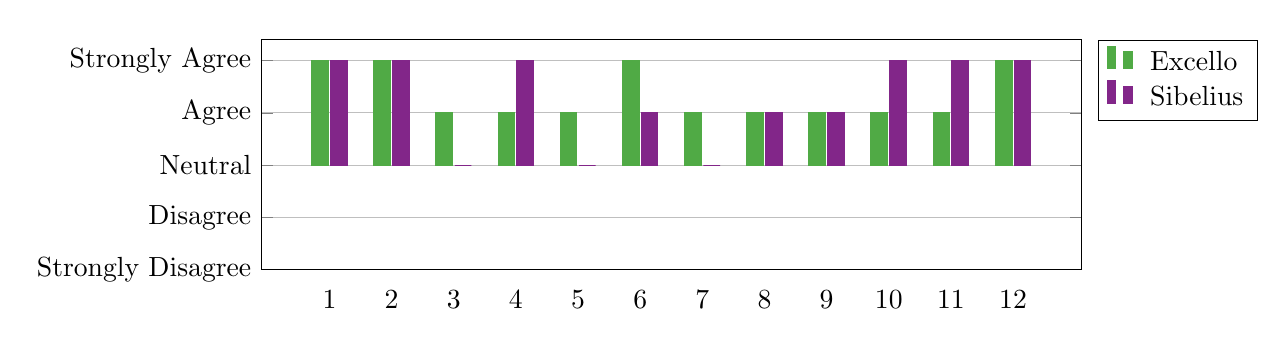
\begin{tikzpicture}
    \begin{axis}[
      % width  = \textwidth,
      width = 12cm,
      height = 4.5cm,
      major x tick style = transparent,
      ybar=2*\pgflinewidth,
      bar width=6pt,
      ymajorgrids = true,
      % ylabel = {Frequency},
      % %xlabel = {Likert Scale Result},
      % symbolic y coords= {-2,-1,0,1,2},
      yticklabels = {Strongly Disagree,Disagree,Neutral,Agree,Strongly Agree},
      xtick = {1,2,3,4,5,6,7,8,9,10,11,12},
      ytick = {-2,-1,0,1,2},
      ymin = -2,
      x tick label style  = {text width=2cm,align=center},
      scaled y ticks = false,
      % enlarge x limits=0.25,
      legend cell align=left,
      legend style={
              at={(1.02,1)},
              anchor=north west,
              column sep=1ex
      }
    ]

    \addplot[style={excelGreen,fill=excelGreen,mark=none}]
    	coordinates {(1,2) (2,2) (3,1) (4,1) (5,1) (6,2) (7,1) (8,1) (9,1) (10,1) (11,1) (12,2) };
    \addplot[style={sibPurple,fill=sibPurple,mark=none}]
    	coordinates {(1,2) (2,2) (3,0) (4,2) (5,0) (6,1) (7,0) (8,1) (9,1) (10,2) (11,2) (12,2) };

    \legend{Excello,Sibelius}

    \end{axis}
\end{tikzpicture}
\caption{User responses for \textit{consistency} for Excello and Sibelius from (b)}
\label{evaluation:cons}
\end{figure}

\subsection{Secondary Notation}

\paragraph{} Given the time spent translating, secondary notation is particularly important~\cite{blackwell:notation}. As Excello abstracts time from the grid axes, the parts distribution is up to the user and cells can be used for arbitrary marks. Therefore, existing Excel features for formatting and grouping cells remain available. This is utilised by the automatic highlighting of notes and turtles. A test value of 15.5 for 8 changed pairs suggests no significant difference in population means. This suggests that the spreadsheet paradigm can provide equal secondary notation abilities to Sibelius, software already equipped with numerous ways to customise a score.

\begin{figure}[tbh]
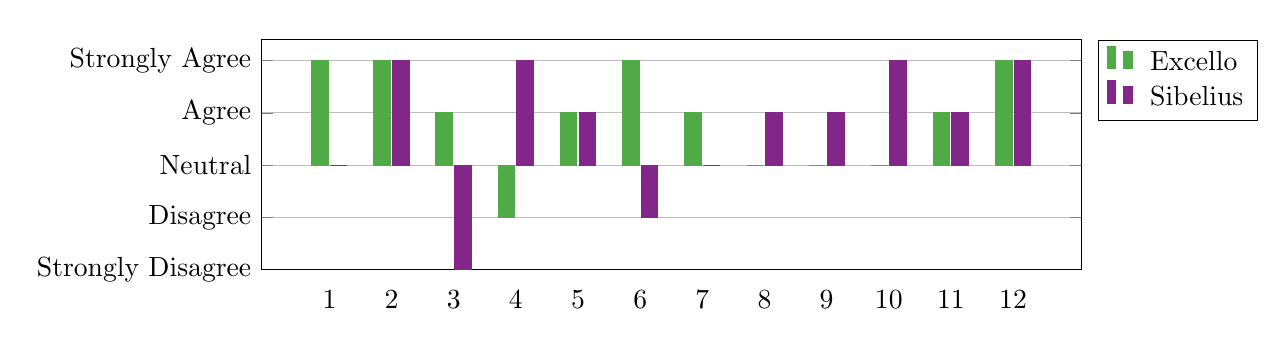
\begin{tikzpicture}
    \begin{axis}[
      % width  = \textwidth,
      width = 12cm,
      height = 4.5cm,
      major x tick style = transparent,
      ybar=2*\pgflinewidth,
      bar width=6pt,
      ymajorgrids = true,
      % ylabel = {Frequency},
      % %xlabel = {Likert Scale Result},
      % symbolic y coords= {-2,-1,0,1,2},
      yticklabels = {Strongly Disagree,Disagree,Neutral,Agree,Strongly Agree},
      xtick = {1,2,3,4,5,6,7,8,9,10,11,12},
      ytick = {-2,-1,0,1,2},
      ymin = -2,
      x tick label style  = {text width=2cm,align=center},
      scaled y ticks = false,
      % enlarge x limits=0.25,
      legend cell align=left,
      legend style={
              at={(1.02,1)},
              anchor=north west,
              column sep=1ex
      }
    ]

    \addplot[style={excelGreen,fill=excelGreen,mark=none}]
      coordinates {(1,2) (2,2) (3,1) (4,-1) (5,1) (6,2) (7,1) (8,0) (9,0) (10,0) (11,1) (12,2) };
    \addplot[style={sibPurple,fill=sibPurple,mark=none}]
      coordinates {(1,0) (2,2) (3,-2) (4,2) (5,1) (6,-1) (7,0) (8,1) (9,1) (10,2) (11,1) (12,2) };

    \legend{Excello,Sibelius}

    \end{axis}
\end{tikzpicture}
\caption{User responses for \textit{secondary notation} for Excello and Sibelius from (c)}
\label{evaluation:secn}
\end{figure}

\subsection{Viscosity}

\paragraph{} Letting dynamics and octave marking be omitted and turtles stepping forward automatically, provides low resistance to making additions and changes to the music. The toggle activation button dramatically reduces the actions to turn turtles on and off. Furthermore, Excel provides easy editing and movement of cells. A test value of 10.5 for 9 changed pairs is not a significant result. This suggests the interfaces have comparable viscosity.

\begin{figure}[tbh]
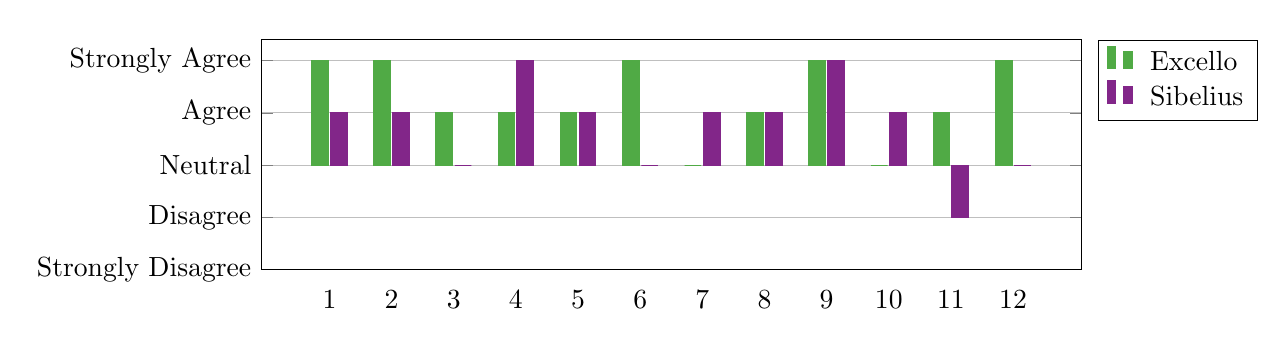
\begin{tikzpicture}
    \begin{axis}[
      % width  = \textwidth,
      width = 12cm,
      height = 4.5cm,
      major x tick style = transparent,
      ybar=2*\pgflinewidth,
      bar width=6pt,
      ymajorgrids = true,
      % ylabel = {Frequency},
      % %xlabel = {Likert Scale Result},
      % symbolic y coords= {-2,-1,0,1,2},
      yticklabels = {Strongly Disagree,Disagree,Neutral,Agree,Strongly Agree},
      xtick = {1,2,3,4,5,6,7,8,9,10,11,12},
      ytick = {-2,-1,0,1,2},
      ymin = -2,
      x tick label style  = {text width=2cm,align=center},
      scaled y ticks = false,
      % enlarge x limits=0.25,
      legend cell align=left,
      legend style={
              at={(1.02,1)},
              anchor=north west,
              column sep=1ex
      }
    ]

    \addplot[style={excelGreen,fill=excelGreen,mark=none}]
    	coordinates {(1,2) (2,2) (3,1) (4,1) (5,1) (6,2) (7,0) (8,1) (9,2) (10,0) (11,1) (12,2) };
    \addplot[style={sibPurple,fill=sibPurple,mark=none}]
    	coordinates {(1,1) (2,1) (3,0) (4,2) (5,1) (6,0) (7,1) (8,1) (9,2) (10,1) (11,-1) (12,0) };

    \legend{Excello,Sibelius}

    \end{axis}
\end{tikzpicture}
\caption{User responses for \textit{viscosity} for Excello and Sibelius from (d)}
\label{evaluation:visc}
\end{figure}

\subsection{Visibility / Juxtaposition}

\paragraph{} For both questions, there was no significant difference in population mean with test values of 6 and 7 for 6 and 7 changed pairs. This suggests that the spreadsheet interface can provide a similar ability to view components to Sibelius.

\begin{figure}[tbh]
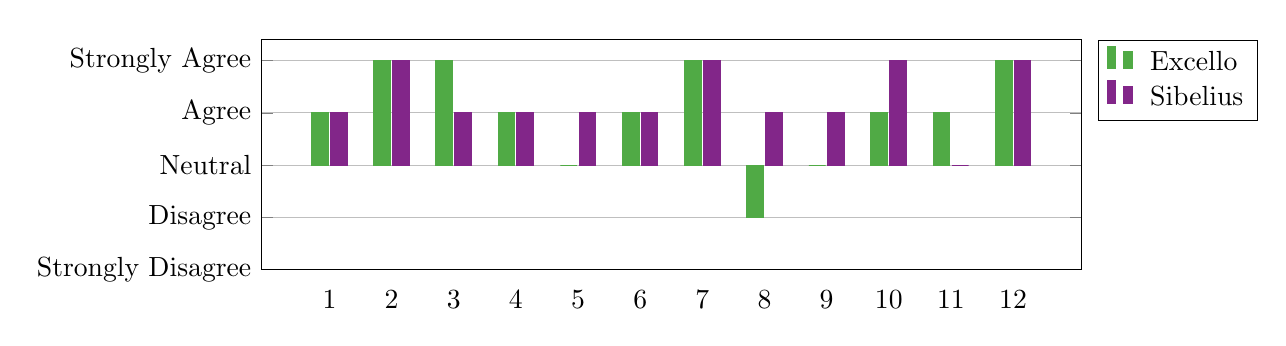
\begin{tikzpicture}
    \begin{axis}[
      % width  = \textwidth,
      width = 12cm,
      height = 4.5cm,
      major x tick style = transparent,
      ybar=2*\pgflinewidth,
      bar width=6pt,
      ymajorgrids = true,
      % ylabel = {Frequency},
      % %xlabel = {Likert Scale Result},
      % symbolic y coords= {-2,-1,0,1,2},
      yticklabels = {Strongly Disagree,Disagree,Neutral,Agree,Strongly Agree},
      xtick = {1,2,3,4,5,6,7,8,9,10,11,12},
      ytick = {-2,-1,0,1,2},
      ymin = -2,
      x tick label style  = {text width=2cm,align=center},
      scaled y ticks = false,
      % enlarge x limits=0.25,
      legend cell align=left,
      legend style={
              at={(1.02,1)},
              anchor=north west,
              column sep=1ex
      }
    ]

    \addplot[style={excelGreen,fill=excelGreen,mark=none}]
    	coordinates {(1,1) (2,2) (3,2) (4,1) (5,0) (6,1) (7,2) (8,-1) (9,0) (10,1) (11,1) (12,2) };
    \addplot[style={sibPurple,fill=sibPurple,mark=none}]
    	coordinates {(1,1) (2,2) (3,1) (4,1) (5,1) (6,1) (7,2) (8,1) (9,1) (10,2) (11,0) (12,2) };

    \legend{Excello,Sibelius}

    \end{axis}
\end{tikzpicture}
\caption{User responses for \textit{visibility/juxtaposition} for Excello and Sibelius from (e)}
\label{evaluation:viju1}
\end{figure}

\begin{figure}[tbh]
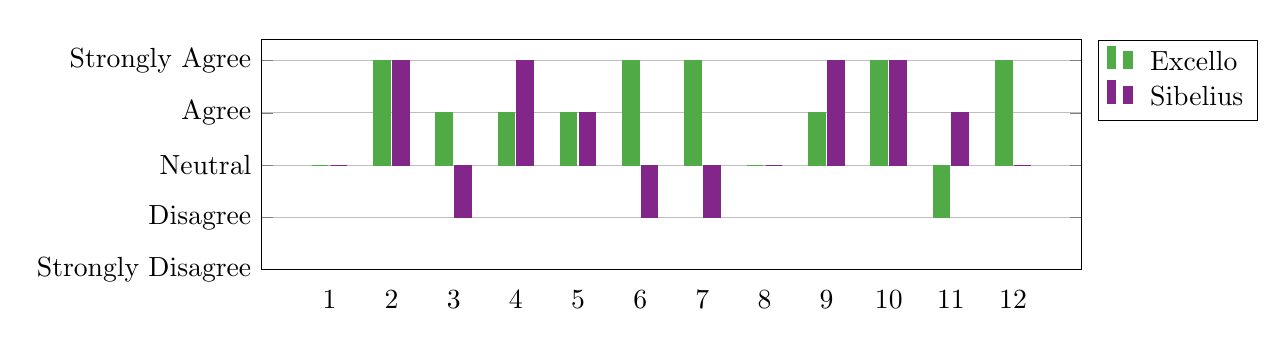
\begin{tikzpicture}
    \begin{axis}[
      % width  = \textwidth,
      width = 12cm,
      height = 4.5cm,
      major x tick style = transparent,
      ybar=2*\pgflinewidth,
      bar width=6pt,
      ymajorgrids = true,
      % ylabel = {Frequency},
      % %xlabel = {Likert Scale Result},
      % symbolic y coords= {-2,-1,0,1,2},
      yticklabels = {Strongly Disagree,Disagree,Neutral,Agree,Strongly Agree},
      xtick = {1,2,3,4,5,6,7,8,9,10,11,12},
      ytick = {-2,-1,0,1,2},
      ymin = -2,
      x tick label style  = {text width=2cm,align=center},
      scaled y ticks = false,
      % enlarge x limits=0.25,
      legend cell align=left,
      legend style={
              at={(1.02,1)},
              anchor=north west,
              column sep=1ex
      }
    ]

    \addplot[style={excelGreen,fill=excelGreen,mark=none}]
    	coordinates {(1,0) (2,2) (3,1) (4,1) (5,1) (6,2) (7,2) (8,0) (9,1) (10,2) (11,-1) (12,2) };
    \addplot[style={sibPurple,fill=sibPurple,mark=none}]
    	coordinates {(1,0) (2,2) (3,-1) (4,2) (5,1) (6,-1) (7,-1) (8,0) (9,2) (10,2) (11,1) (12,0) };

    \legend{Excello,Sibelius}

    \end{axis}
\end{tikzpicture}
\caption{User responses for \textit{visibility/juxtaposition} for Excello and Sibelius from (f)}
\label{evaluation:viju2}
\end{figure}

\paragraph{} Sibelius uses established music notation as part of professional software. However, there was no significant evidence to suggest Sibelius outperformed Excello across the CDN. This suggests that despite being a general purpose spreadsheet environment, Excello is a successful interface for writing music.

\subsection{Other Dimensions}

\paragraph{} If users are unfamiliar with the turtle paradigm, this may reduce the \textit{role-expressiveness}. But turtles and notes are the only musical spreadsheet components and are identified by highlighting. Whilst notes and turtles can be added in any order, adding parts may require many line insertions, increasing the \textit{premature commitment}. The dual-formalism of turtles and notes could create high \textit{diffuseness} but the layout flexibility allows this to be minimized as in Figure \ref{evaluation:excelloFranzRedacted}. This also shows how representations can have strong \textit{synopsie}, as the notes or turtles don't need to be examined to understand what is happening. This may come at the expense of \textit{hidden dependencies} if it is not immediately clear which notes are triggered by which turtles. Volume is also dependent on the notes turtles play before it. But as a single cell could be played at multiple volumes, this is a tradeoff of this design decision.

\paragraph{} As well as the ``\texttt{m*}" notation decreasing \textit{viscosity}, it also improves the \textit{progressive evaluation} as turtles can be played before a whole part has been transcribed. The ability to define a turtle and fill in the notes later also improves the \textit{provisionality}. ``\texttt{m*}" also reduces \textit{hard mental operations} and the chord input tool removes manual calculation of the notes of chords.

\paragraph{} Spreadsheets are ``an abstraction-hating system"~\cite{blackwell:tutorial}, therefore little \textit{abstraction} is provided by Excel, grouping turtles in one definition and nested bracketing of movement instructions improve this. These features also provide good \textit{legibility}.

\section{Ethics and Data Handling}

\paragraph{} After ethics approval, the pilot formative evaluation session was designed. After the pilot (also performed for summative evaluation), the session was revised before continuing with the remaining sessions. Participants filled in a consent form explaining the project and the session format. Participants had the choice to remain anonymous and not appear in acknowledgements. All participants' data included a unique ID to use to request removal or anonymising of their data. All participant data was only seen by myself. Formative evaluation sessions were audio recorded, typed up after the session, and then the audio was deleted. All participant data was also backed up on GitHub with the rest of the project but in an encrypted folder. Physical backups were also encrypted.
